\chapter{High Dynamic Range Imaging}\label{ch:hdr-imaging}

Photographers have long understood that the range of brightness levels in
a real-world scene is considerably larger than the range that can be
captured by a camera's film or imaging sensor.  The luminance of a
outdoor scene can easily span five orders of magnitude, however
typical digital cameras encode the brightness at a single pixel
location using a modest 8-bits (2 orders of magnitude).  Pixels that
fall outside the {\em dynamic range} of the camera sensor will either
be underexposed or overexposed; their values will be at the minimum or
maximum pixel value of the camera, respectively.

Some digital cameras can save RAW images with higher dynamic range.
These cameras can capture 12 bits per pixel, or 4096 brightness
levels.  This expanded dynamic range is often sufficient to capture
scenes with a moderate amount of contrast. However, to capture scenes
with very high dynamic range, you must generate a HDR image from a set
of {\em bracketed} exposures: a group of low dynamic range images of
the exact same scene taken with different exposure settings that vary
from under-exposed to over-exposed.  This technique is subject of
section \ref{sec:hdr_merge}.

The resulting HDR image is generally stored with a channel type of
{\tt float} or {\tt int16} to accommodate the expanded dynamic range.
To store HDR images on disk we recommend using the OpenEXR or TIFF
file formats, both of which support 32-bit floating point channel
types.

Just as capturing HDR images can be challenging, visualizing them is
also difficult.  Print media and most display devices can only manage
about 2 orders of magnitude of dynamic range, whereas an HDR image may
have 5 or more orders of magnitude. Simply scaling the image to the
display range will cause it to look overly dark or washed-out. Section
\ref{sec:tonemapping} discusses a technique called {\em tone mapping}
that reduces the dynamic range of an image while preserving as much as
possible the visual contrasts of the original scene.

\section{Merging Bracketed Exposures}
\label{sec:hdr_merge}

As discussed in the introduction to this chapter, the limited dynamic
range of the sensors on modern cameras necessitates a different
strategy for building true HDR images: exposure bracketing.  This frees
us from hardware limitations and allows us to set the dynamic range of
the output image arbitrarily by adjusting the number of exposures in
the bracket.  The more exposures in the bracket, the higher the
dynamic range merged HDR image.

\begin{figure}[tbp]
\begin{center}
  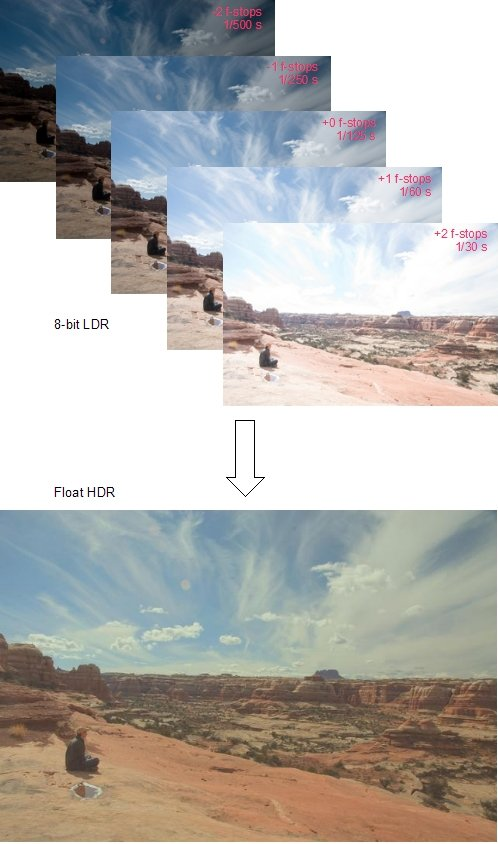
\includegraphics[width=5in]{images/hdr_merge.jpg}
 \end{center}
  \caption{A stack of 8-bit-per-channel LDR images separated by one
    f-stop is merged a floating-point HDR image. The HDR image is
    tone-mapped for display using the Drago operator.}
  \label{fig:hdrmerge}
\end{figure}

For convenience, the exposure ratio between consecutive images is
usually a fixed value to guarantee a wide exposure range while
maintaining even brightness overlap between adjacent images in the
bracket. A factor of two is generally recommended.  The shutter speed
is generally the preferred method of varying the exposure in a
bracket; changing the aperture or ISO setting can have the same effect
on exposure but they may change the focus or increase noise.

\subsection{Converting LDR Images to an HDR Image}
The HDR module has a set of free functions that make stitching a stack
of LDR images into an HDR image as simple as one function
call. \verb#process_ldr_images()# (in \verb#<vw/HDR/LDRtoHDR.h>#)
takes a \verb#std::vector# of ImageViews (with grayscale or RGB pixels
and a floating point channel type), sorted from darkest to
brightest. This function assumes a constant exposure ratio between
images; it can be specified or the default value of $\sqrt{2}$ can be
used (corresponding to 1 f-stop, or a power of two in shutter
speed). An overloaded version accepts a \verb#std::vector<double># of
absolute brightness values for each image (as defined by the APEX
system \cite{apex}) .

\begin{verbatim}
  // Generate HDR image from HDR stack. 
  vector<ImageView<PixelRGB<double> > > images(num_images);
  
  // ... Read input images ...

  // Assum default exposure ratio
  ImageView<PixelRGB<double> > hdr_image = process_ldr_images(images);
\end{verbatim}

Most modern digital cameras store exposure information as EXIF
metadata in the headers of images.  The Vision Workbench supports
reading this data from TIFF and JPEG files via the Camera Module, and
the routine \verb#process_ldr_images_exif()# capitalizes on this,
generating an HDR image from an array of filenames of LDR images by
computing brightness values from the files' EXIF data along the
way. 

%% \subsection{Alignment}
%% It is crucial for the images in an HDR stack to be aligned, both so
%% that the resulting HDR image is not blurry and so that the camera
%% response curve can be estimated accurately.  The best solution is to
%% take the HDR stack on a tripod, ideally using remote capture.  {\em If
%%   you are able to take the images on a stationary platform, there is
%%   no need to perform image alignment in software.}  However, for
%% handheld photographs, or if dynamic disturbances, such as wind, shake
%% the camera on the tripod, software alignment is then likely to be
%% necessary.

%% For HDR stacks shot with a hand-held camera or otherwise unaligned,
%% the HDR module includes MTBAlign.h, an implementation of the Mean
%% Threshold Bitmap (although it actually uses the median) alignment
%% technique \cite{hdrbook}. MTB alignment thresholds two images on their
%% respective medians and finds the x- and y-shifts that minimize the
%% difference of the resulting bitmaps. This technique is well-suited for
%% HDR stacks as the median threshold bitmap is relatively invariant with
%% respect to the exposure used to take the photo, whereas edges may fade
%% in and out. The weakness of MTB alignment is that it only considers
%% translation. This should be sufficient even for most photos taken
%% hand-held, but to align images that are rotated or otherwise warped, a
%% more sophisticated alignment technique should be used (the
%% InterestPoint module, for example).

%% \begin{verbatim}
%% // Find the shift to be applied to img2 to match it most
%% // closely with img1.

%% int shift_bits = 6; // Maximum shift of 64 pixels
%% int shift[2];       // Will hold (x,y) shift

%% // img1 and img2 assumed to be of type
%% // ImageView<PixelGray<double> >.
%% get_exp_shift(img1, img2, shift_bits, shift);
%% \end{verbatim}

\subsection{The Camera Response Curves}
The relationship between light entering a camera sensor and the pixel
value that is recorded in the image is a non-linear.  It depends on
many factors, including the degree of gamma correction used in the
image, the color balance across the range of brightness, and the
camera's post processing settings (especially contrast).  The function
that encompasses all of these and maps the amount of light on the
sensor (the luminance) to the pixel value is referred to as the camera
response curve.  See Figure \ref{fig:hdr_camera_curve} for an example.

\begin{figure}[tbp]
\begin{center}
  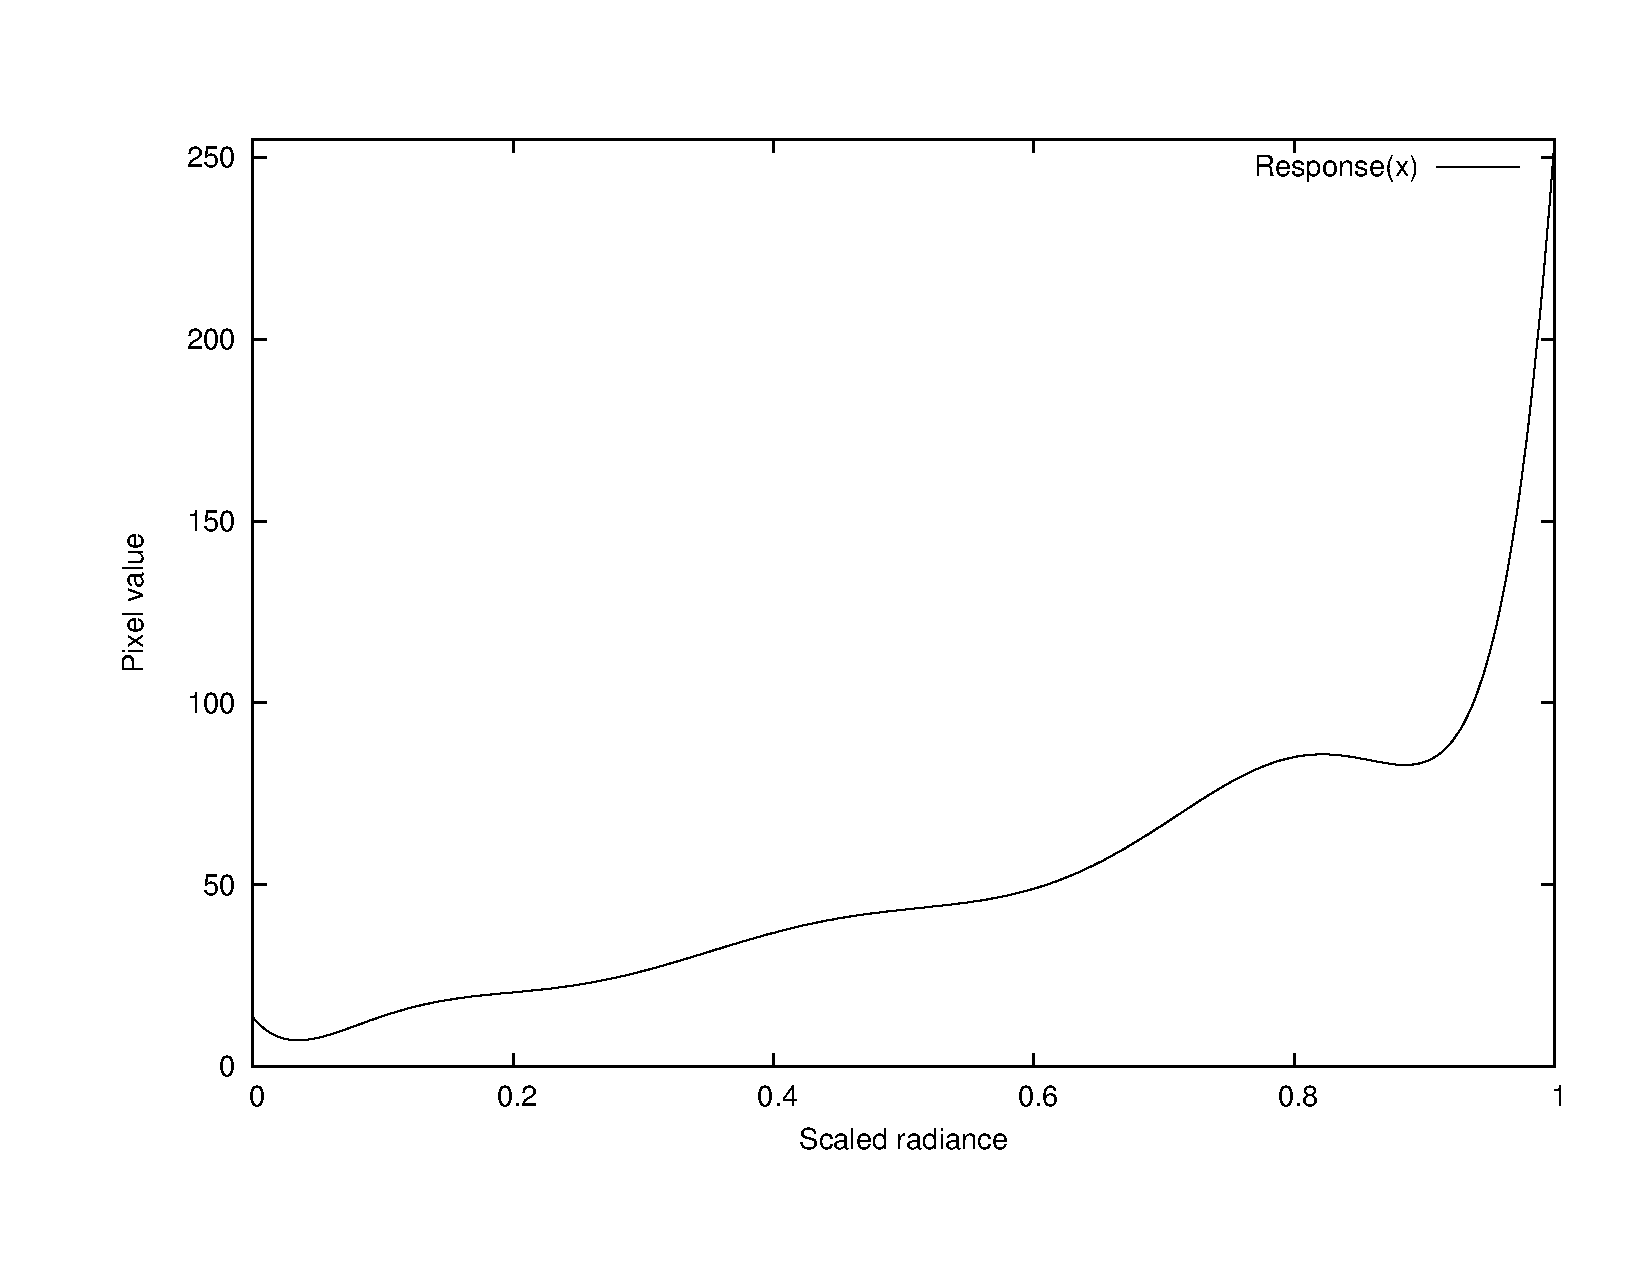
\includegraphics[width=5in]{images/hdr_response.pdf}
 \end{center}
  \caption{Camera response curve estimated from an HDR stack.}
  \label{fig:hdr_camera_curve}
\end{figure}

To create a HDR image that truly represent the physical brightness
levels in a scene, it is necessary to estimate the inverse of the
camera response curves (we assume a separate curve for each channel)
and apply it to the image data.  That is, we would like to find a
function that, given a pixel value in the image and its exposure
information, returns the luminance of the scene at that point.
\verb#<vw/HDR/CameraCurve.h># implements
\verb#estimate_inverse_camera_curve()#, a free function that estimates
the inverse response curve as a polynomial.  This routine takes a
matrix of aligned pixel channel values from an HDR stack and their
brightness ratios. This function is used internally by
\verb#LDRtoHDR.h#; most users will probably not need to call it
directly.

The CameraCurve sources also supply \verb#invert_curve()#, a free
function that approximates the inverse of a polynomial curve, also as
a polynomial. This is useful to recover the actual camera response
curve (mapping a scaled luminance value to a pixel value) from the
inverse response curve determined by
\verb#estimate_inverse_camera_curve()#. Re-applying the camera
response curve to an HDR image after tone-mapping can improve the
colors and overall visual appeal. See the code in
Listing~\ref{lst:ExifHDRExample.cc} for an example.

\begin{figure}[tbp]
\begin{center}
  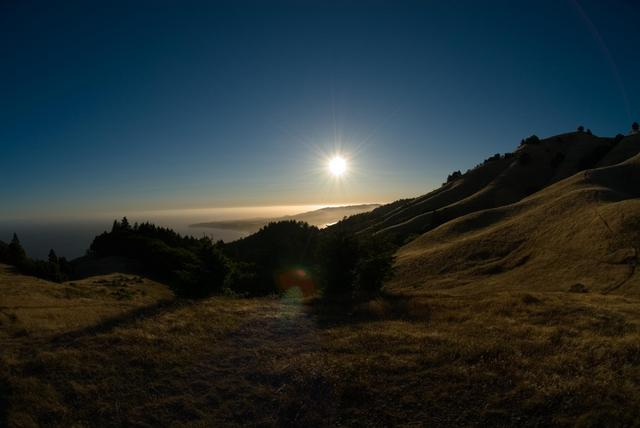
\includegraphics[height=3in]{images/hdr_original.jpg}
  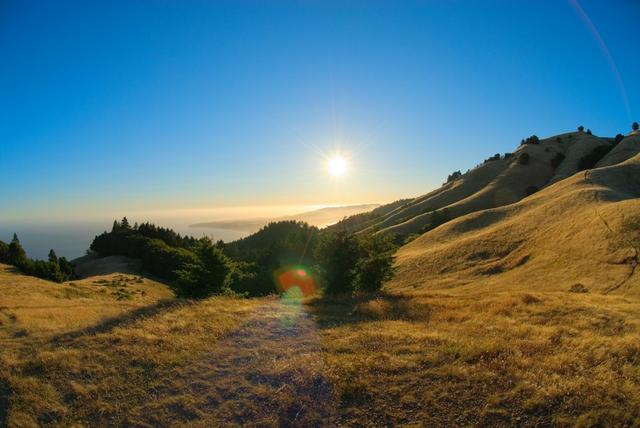
\includegraphics[height=3in]{images/hdr_drago.jpg}
  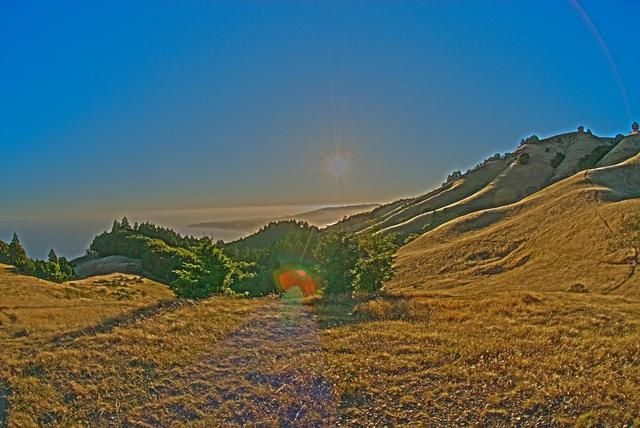
\includegraphics[height=3in]{images/hdr_ashikhmin.jpg}
 \end{center}
  \label{fig:tonemapping}
  \caption{Top: an image taken in 12-bit RAW format. Middle: after
           tone-mapping with the Drago operator. Bottom: after
           tone-mapping with the Ashikhmin operator.}
\end{figure}

\section{Tone Mapping}
\label{sec:tonemapping}
Since print media and most display technologies are inherently LDR,
the dynamic range of a HDR image must be compressed before it
can be displayed. Simply scaling the pixel luminances linearly
yields poor results because the human visual system's response to
luminance is approximately logarithmic rather than linear. A linear
scaling tends to lose small details and local contrast, and the
image as a whole will appear under or over-exposed.

A wide variety of tone-mapping operators have been proposed to
compress the dynamic range of a HDR image while preserving
details and local contrast as much as possible. Using an ideal
tone-mapping operator, the observer of a tone-mapped LDR image
would have a perceptual response matching that of the original
HDR scene. Due to its greater realism, tone-mapping can
vastly improves the appearance of the displayed image.

There are several broad classes of tone-mapping operators, including
global operators, local operators, and operators that use the
gradient or frequency domains. The HDR module currently includes
one global operator and one local operator; they are described in
the following sections.

\subsection{Global Operators}
Global tone-mapping operators apply the same compressive function to
all pixels in the image. Such operators are implemented in
\verb#<vw/HDR/GlobalToneMap.h>#. Currently one such operator is implemented, the
Drago Adaptive Logarithmic Mapping operator.  For algorithm details
see \emph{High Dynamic Range Imaging} \cite{hdrbook} or the original
paper \cite{drago}.  The Drago operator is currently the operator of
choice in the HDR module. It is quite fast, produces good results for
a wide range of images, and can usually be used with its parameters at
default values. Optionally, the parameters bias (controlling contrast,
usually between 0.7 and 0.9), exposure factor (a simple multiplier to
control the overall brightness of the image), and max display
luminance (usually about 100) can be specified.

\begin{verbatim}
  // Apply Drago tone-mapping operator 
  ImageView<PixelRGB<float> > tone_mapped = drago_tone_map(hdr_image);
\end{verbatim}

\subsection{Local Operators}
Local tone-mapping operators compress a pixel's dynamic range in a way
dependent on the neighborhood of pixels around it. These operators
mimic the local adaptation of the human eye and are capable of more
striking or artistic results than global operators, but they are also
susceptible to artifacts such as excessive haloing and reverse
gradients. \verb#<vw/HDR/LocalToneMap.h># currently implements the Ashikhmin local
tone-mapping operator \cite{ashikhmin}.  It is much slower than the
Drago operator and more prone to artifacts, but may be useful for some
images. Its only parameter is a threshold value (0.5 by default) which
roughly controls the size of the neighborhood used for each pixel. A
threshold value too large will result in haloing.

\begin{verbatim}
  // Apply Ashikhmin tone-mapping operator 
  ImageView<PixelRGB<float> > tone_mapped = ashikhmin_tone_map(hdr_image);
\end{verbatim}

%% \section{Panoramic HDR}
%% Applying HDR techniques to panoramic images is extremely challenging,
%% as it is necessary to consider how each individual image is placed in
%% the full panorama.  LDRtoHDRPano.h contains prototype code for
%% computing the response curves from a set of panoramic images and
%% projecting the individual images into the same luminance
%% space. Blending the resulting images together into a full panorama is
%% left to a separate blender.

%% The difficult part is computing the camera response curves from the
%% panoramic images; it would be simpler to compute and cache the
%% response curves using a standard HDR stack, but on digital cameras the
%% response curves may vary with settings. Basically, the areas of the
%% panorama where two or more individual images overlap are used as HDR
%% stacks for sampling. The panorama is traversed considering one square
%% section at a time, so that only those images overlapping that section
%% need to be loaded (keeping all of the individual images in memory at
%% once would be too memory-inefficient).  Brightness data is extracted
%% from the Exif data in the original images.

%% LDRtoHDRPano.h defines the free function
%% process\_ldr\_images\_pano. The inputs will likely need to be changed
%% to accept whatever variety of ImageView(Ref) the panorama alignment
%% algorithm produces. Currently the inputs are a vector of PanoImage
%% structs, an optional vector of brightness values for the images
%% (otherwise Exif is used), the width and height of the full panorama,
%% and a vector of vw::Vectors to store the computed camera response
%% curves. PanoImage holds the image's file name, a Rect struct which
%% holds its dimensions and offset within the panorama, and a
%% brightness\_multiplier field in which process\_ldr\_images\_pano
%% stores a multiplier that will project the image into the same
%% luminance space as the others (after applying the camera curves using
%% the function psi from LDRtoHDR.h). The outputs are the camera response
%% curves and the brightness multipliers.


%% \begin{verbatim}
%% /* Create a PanoImage struct */
%% PanoImage img = PanoImage(``img.jpg'', Rect(img_x,
%%                 img_y, width, height), 0);

%% /* Compute response curves and brightness multipliers */
%% vector<PanoImage> images;
%% vector<Vector<double> > curves;
%% // ... load images ..
%% process_ldr_images_pano(images, pano_width,
%%                         pano_height, curves);
%% \end{verbatim}

\section{Command Line Tools}

The HDR module builds two small utilities for working with HDR images
from the command terminal.  If you simply type these command names
with no arguments, you will see a list of acceptable arguments.

\begin{itemize}
\item \verb#hdr_merge#   : Merge LDR images into one HDR image
\item \verb#hdr_tonemap# : Tonemap an HDR image using the Drago operator
\end{itemize}

\section{Other Resources}
There are a number of freely available utilities which are useful for
working with HDR images. The OpenEXR distribution \cite{openexr}
includes several utilities, including exrdisplay for displaying
OpenEXR images. {\tt exrtools} \cite{exrtools} provides utilities for
converting between OpenEXR and other formats, performing basic
operations on OpenEXR images, and a couple of tone-mapping
utilities. {\tt pfstools} \cite{pfstools} is a well-integrated set of
utilities for reading, writing, manipulating and viewing HDR images.
It has an associated pfstmo project that implements seven of the more
prominent tone mapping operators.

\sourcelst{ExifHDRExample.cc}{ This is a simple test program that
  stitches an Exif-tagged HDR stack into an HDR image, performs
  tone-mapping, and saves several versions with different
  post-processing applied for comparison. Usually the best image is
  produced by re-applying the camera response curves and then gamma
  correcting.}
\begin{verbatim}
\end{verbatim}

\begin{thebibliography}{1}

\bibitem{ashikhmin} Ashikhmin, Michael, ``A Tone Mapping Algorithm for High Contrast Images,''
{\em Eurographics Workshop on Rendering}, 2002: 1--11.

\bibitem{exrtools} Biggs, Billy, ``exrtools: a collection of utilities for manipulating
OpenEXR images,'', 2004, http://scanline.ca/exrtools/.

\bibitem{drago} Drago et al., ``Adaptive Logarithmic Mapping For Displaying High Contrast Scenes,''
{\em Eurographics}, {\bf 22}(3), 2003.

\bibitem{fattal} Fattal, Raanan, et. al, ``Gradient Domain High Dynamic Range Compression,''
{\em ACM Transactions on Graphics}, 2002.

\bibitem{openexr} Industrial Light and Magic, ``OpenEXR,'' (Lucasfilm Ltd., 2006),
http://www.openexr.com.

\bibitem{apex} Kerr, Douglas, ``APEX--The Additive System of Photographic Exposure,'' 2006,
http://doug.kerr.home.att.net/pumpkin/APEX.pdf.

\bibitem{pfstools} Mantiuk, Rafal, and Grzegorz Krawczyk, ``pfstools for HDR processing,'' 2006,
http://www.mpi-inf.mpg.de/resources/pfstools/.

\bibitem{reinhard} Reinhard, Erik, et. al. ``Photographic Tone Reproduction for Digital Images,''
{\em ACM Transactions on Graphics}, 2002.

\bibitem{hdrbook} Reinhard, Erik, Greg Ward, Sumanta Pattanaik, and Paul Debevec,
{\em High Dynamic Range Imaging}, (Boston: Elsevier, 2006).

\bibitem{ward} Ward, Greg, et al., ``A Visibility Matching Tone Reproduction Operator for High Dynamic Range Scenes,''
{\em IEEE Transactions on Visualization and Computer Graphics}, 1997.

\end{thebibliography}
